\documentclass[border=10pt]{standalone}
\usepackage{tikz}
\usetikzlibrary{shapes.geometric, arrows.meta, positioning, calc, fit, backgrounds}
\usepackage{amsmath}

\begin{document}
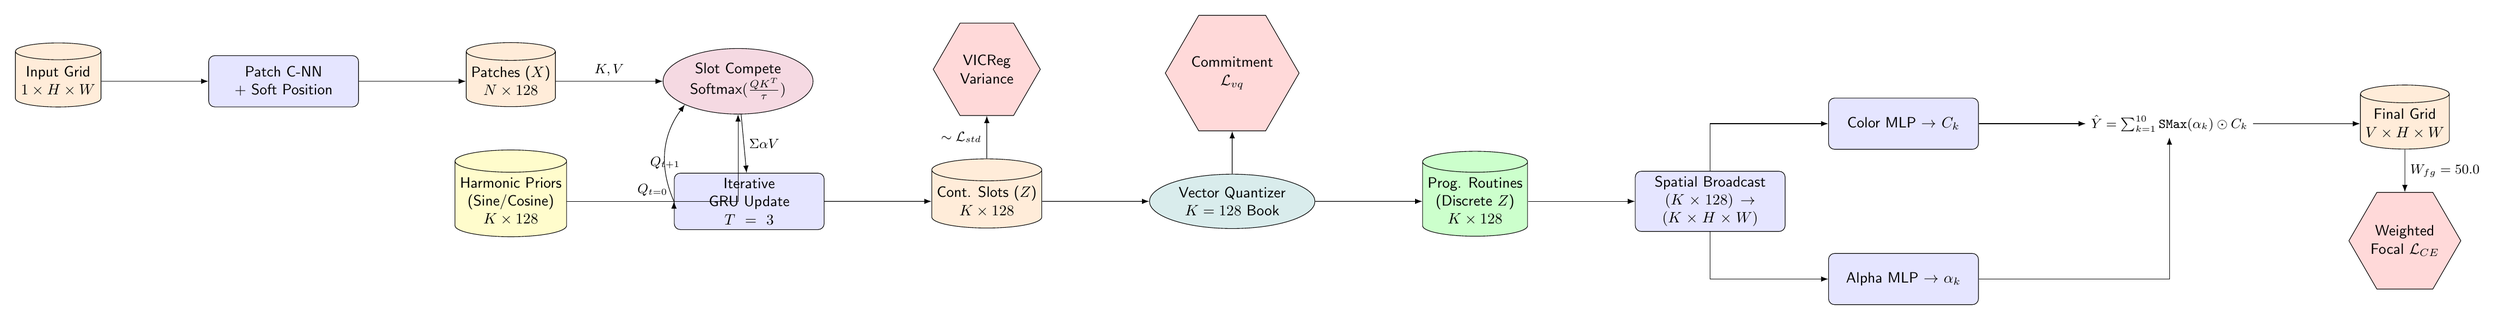
\begin{tikzpicture}[
    >=Latex,
    node distance=1.5cm and 2.5cm,
    font=\sffamily,
    % Styles
    data/.style={draw, cylinder, shape aspect=0.2, shape border rotate=90, minimum width=2cm, minimum height=1.5cm, align=center, fill=orange!15},
    block/.style={draw, rectangle, rounded corners, minimum width=3.5cm, minimum height=1.2cm, align=center, fill=blue!10, text width=3cm},
    attn/.style={draw, ellipse, minimum width=3cm, minimum height=1.2cm, align=center, fill=purple!15},
    loss/.style={draw, regular polygon, regular polygon sides=6, inner sep=0pt, minimum size=2.5cm, align=center, fill=red!15},
    math/.style={align=center, font=\ttfamily\small}
]

% 1. Input Layer
\node[data] (input) {Input Grid \\ $1 \times H \times W$};
\node[block, right=of input] (patch) {Patch C-NN \\ + Soft Position};
\node[data, right=of patch] (patches) {Patches ($X$) \\ $N \times 128$};

\draw[->] (input) -- (patch);
\draw[->] (patch) -- (patches);

% 2. Slot Initialization
\node[data, below=1cm of patches, fill=yellow!20] (priors) {Harmonic Priors \\ (Sine/Cosine) \\ $K \times 128$};
\node[block, right=of priors] (gru) {Iterative GRU Update \\ $T=3$};

% 3. Attention Mechanism
\node[attn, right=of patches] (slotattn) {Slot Compete\\ $\text{Softmax}(\frac{QK^T}{\tau})$};

\draw[->] (patches) -- node[above, math] {$K, V$} (slotattn);
\draw[->] (priors) -| node[near start, above, math] {$Q_{t=0}$} (slotattn);
\draw[->] (slotattn) -- node[right, math] {$\Sigma \alpha V$} (gru);
\draw[->] (gru.west) edge[bend left=30] node[below, math] {$Q_{t+1}$} (slotattn.south west);

% 4. Continuous Latents and VQ
\node[data, right=of gru] (zcont) {Cont. Slots ($Z$) \\ $K \times 128$};
\node[loss, above=1cm of zcont] (vicreg) {VICReg \\ Variance};
\node[attn, right=of zcont, fill=teal!15] (vq) {Vector Quantizer \\ $K=128$ Book};
\node[loss, above=1cm of vq] (vqloss) {Commitment \\ $\mathcal{L}_{vq}$};
\node[data, right=of vq, fill=green!20] (zdisc) {Prog. Routines \\ (Discrete $Z$) \\ $K \times 128$};

\draw[->] (gru) -- (zcont);
\draw[->] (zcont) -- (vicreg) node[midway, left, math] {$\sim \mathcal{L}_{std}$};
\draw[->] (zcont) -- (vq);
\draw[->] (vq) -- (zdisc);
\draw[->] (vq) -- (vqloss);

% 5. Decoder Phase
\node[block, right=of zdisc] (broadcast) {Spatial Broadcast \\ $(K \times 128) \rightarrow (K \times H \times W)$};
\node[block, above right=0.5cm and 1cm of broadcast] (colormlp) {Color MLP $\rightarrow C_k$};
\node[block, below right=0.5cm and 1cm of broadcast] (alphamlp) {Alpha MLP $\rightarrow \alpha_k$};

\draw[->] (zdisc) -- (broadcast);
\draw[->] (broadcast) |- (colormlp);
\draw[->] (broadcast) |- (alphamlp);

% 6. Reassembly
\node[math, right=of colormlp] (sum) {$\hat{Y} = \sum_{k=1}^{10} \text{SMax}(\alpha_k) \odot C_k$};
\draw[->] (colormlp) -- (sum);
\draw[->] (alphamlp) -| (sum);

% 7. Output & Final Loss
\node[data, right=of sum] (output) {Final Grid \\ $V \times H \times W$};
\node[loss, below=1cm of output] (celoss) {Weighted \\ Focal $\mathcal{L}_{CE}$};

\draw[->] (sum) -- (output);
\draw[->] (output) -- (celoss) node[midway, right, math] {$W_{fg}=50.0$};

\end{tikzpicture}
\end{document}
